\documentclass[12pt]{report}
% USER PACKAGE
\usepackage{graphicx}
\usepackage[italian]{babel}
\usepackage{hyperref}
\usepackage{subcaption}
\usepackage{float}
\usepackage{caption}
\usepackage{listings}
\usepackage{amsmath}
\usepackage[table]{xcolor}
\usepackage{pgfplots}
\usepackage{graphicx}
\usepackage{textcomp}
\usepackage{titlesec}
\usepackage[parfill]{parskip}
\usepackage[cache=false]{minted}
\usemintedstyle{monokai}

\setcounter{secnumdepth}{4}
\setcounter{tocdepth}{4}



% OTHER SETTINGS
\hypersetup{colorlinks = true, linkcolor = blue}
\pagenumbering{gobble}
\usepackage{geometry}
\geometry{a4paper, top=2cm, bottom=2cm}
\pgfplotsset{compat=1.15}

% REMOVE 1ST PAGE----------------------------------------------
  %  \usepackage{atbegshi} % http://ctan.org/pkg/atbegshi 
  %  \AtBeginDocument{\AtBeginShipoutNext{\AtBeginShipoutDiscard}}
% -------------------------------------------------------------


\title{\textbf{Shadow mapping} \\
    \large Generazione delle ombre in OpenGL
    \begin{figure}[H]
  \centering
    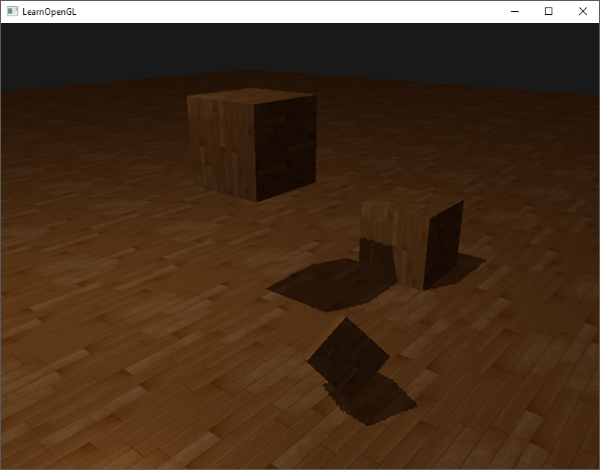
\includegraphics[width=300]{img/copertina_temp.png}
\end{figure}
}

\author{Giovanni Danieli\\
        Laurea Magistrale in Ingegneria e Scienze Informatiche\\
        VR463656\\
            \and
            \\
            \\
        Università degli Studi di Verona\\
        Anno Accademico : 2020/2021
}
\captionsetup[figure]{list=no}
\begin{document}
\addtolength{\topmargin}{-30mm}
\thispagestyle{empty}
\date{}
\maketitle
\pagenumbering{arabic}
\hypersetup{linkcolor  = black}
\tableofcontents
\thispagestyle{empty}
\addtocontents{toc}{~\hfill\textbf{Pagina}\par}
\addtolength{\topmargin}{15mm}
\setlength{\parskip}{1em}

\addtolength{\topmargin}{15mm}
\chapter{Introduzione}

Le ombre, ovvero l'assenza di luce, non sono perfettamente implementabili a causa dell'assenza di algoritmi efficienti nel rendering in tempo reale. Tuttavia esistono molteplici tecniche che offrono buoni risultati per l'approssimazione delle ombre, ognuna però con i propri difetti e problemi che devono essere presi in considerazione.

Una tecnica molto utilizzata nei videogiochi che offre buoni risultati ed è semplice da implementare e non impatta più di tanto la performance è lo \textbf{shadow mapping}; inoltre può evolvere in algoritmi più avanzati come lo \textbf{Omnidirectional Shadow Maps} e lo \textbf{Cascaded Shadow Maps}.

\chapter{Shadow mapping}
L’idea dietro lo Shadow mapping è molto semplice: renderizzare la scena dal punto di vista della luce; tutto quello visibile dal punto di vista della luce è illuminato mentre quello non visibile è in ombra.

\begin{figure}[H]
  \centering
    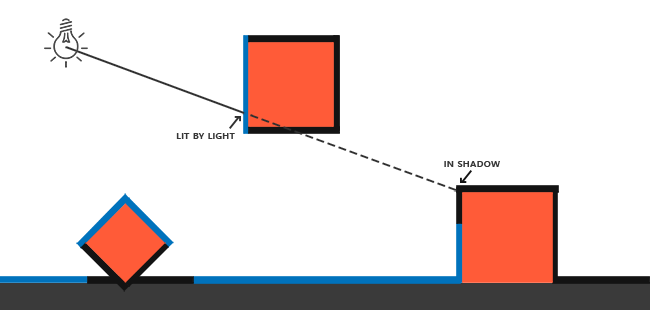
\includegraphics[width=1.0\textwidth]{img/shadow_mapping_theory.png}
\end{figure}
 
Nell’immagine  le linee blu rappresentano i frammenti visibili alla fonte di luce, mentre le linee nere sono nascoste e rappresentano l’ombra. Se tracciamo una retta dalla fonte di luce al cubo più a destra il raggio di luce colpisce prima il cubo fluttuante. Come risultato il frammento del cubo fluttuante è illuminato mentre quello del contenitore più a destra non lo è, risultando in ombra.

Vogliamo ottenere il punto sul raggio dove è avvenuto il primo contatto con un oggetto e confrontarlo con altri punti su questo raggio. Quindi eseguiamo un test di base per vedere se la posizione del raggio di un punto di prova è più lontano dalla fonte rispetto al punto più vicino e, in tal caso, il punto di prova è in ombra. Iterare su possibili migliaia di raggi di luce è un approccio estremamente inefficiente e non si presta bene per il rendering Real Time.

Un approccio migliore e più efficente è renderizzare la scena dal punto di vista della luce e salvare i valori della profondità all'interno di una texture; i valori memorizzati all'interno di questa texture rappresentano i valori di profondità più vicini alla fonte di luce e la texture prende il nome di \textbf{shadow map} o \textbf{depth map}.\\

\begin{figure}[H]
  \centering
    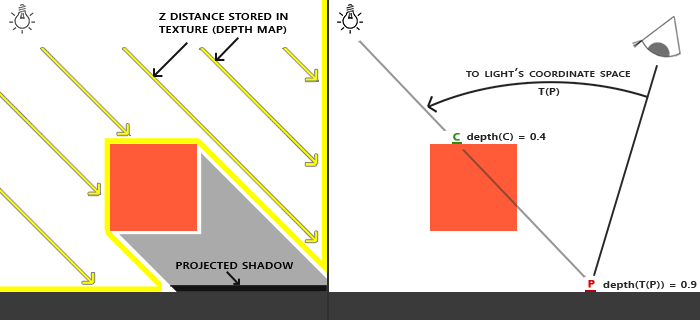
\includegraphics[width=1.0\textwidth]{img/shadow_mapping_theory_spaces.png}
\end{figure}
 
L’immagine a sinistra mostra una fonte di luce direzionale (i raggi sono paralleli tra di loro) proiettare l'ombra del cubo sulla superficie sotto. Usando i valori memorizzati nella depth map troviamo i punti più vicini alla fonte e li utilizziamo per determinare se i frammenti della superficie sotto sono in ombra. Creiamo la depth map renderizzando la scena utilizzando una view matrix e una projection matrix specifiche per quella fonte di luce. Queste matrici insieme formano la matrice \textit{\textbf{T}} che trasformano qualsiasi posizione 3D nello spazio coordinate della fonte di luce.

Nell’immagine a destra vediamo la stessa luce direzionale e la camera. Renderizziamo un frammento nel punto \textit{\textbf{P}} il quale dobbiamo determinare se si trova in ombra o meno. Per prima cosa dobbiamo trasformare il punto \textit{\textbf{P}} nello spazio delle coordinate della luce usando la trasformazione \textit{\textbf{T}}. Ora che il punto \textit{\textbf{P}} è visto dalla prospettiva della luce, la sua coordinata \textit{z} corrisponde alla sua profondità. Usando il punto \textit{\textbf{P}} possiamo indicizzare la depth map per ottenere la profondità più vicina visibile dalla prospettiva della luce, ovvero il punto \textit{\textbf{C}}. Dato che la depth map ritorna una profondità minore rispetto a quello del punto \textit{\textbf{P}}, possiamo concludere che il punto \textit{\textbf{P}} è occluso e quindi in ombra.

Lo shadow mapping quindi consiste in due passaggi: prima renderizziamo la depth map,  successivamente renderizziamo la scena normalmente e usiamo la depth map generata per determinare quali frammenti sono in ombra.

\chapter{Implementazione in OpenGL}
\section{Definizione della depth map}
Come prima cosa generiamo la depth map. Siccome vogliamo solo i valori della profondità specifichiamo il formato della texture come GL\_DEPTH\_COMPONENT. Inoltre diamo alla texture una risoluzione di 1024 x 1024 pixel. Infine attacchiamo la texture al relativo framebuffer.\\
Dato che non abbiamo un color buffer ed abbiamo disabilitato i draw e read buffer, i fragments risultanti non richiedono alcun tipo di elaborazione, quindi usiamo un fragment shader vuoto.

\section{Impostare la trasformazione nello spazio luce}
Una volta definita la depth map dobbiamo impostare le view e projection matrix per renderizzare la scena dal punto di vista della luce. 

Per la projection matrix, usando una luce direzionale dove tutti i raggi di luce sono paralleli, impostiamo una matrice di proiezione ortografica.

\begin{minted}[bgcolor=black]{cpp}
float near_plane = 1.0f, far_plane = 7.5f;
glm::mat4 lightProjection = glm::ortho(-10.0f, 10.0f, -10.0f,10.0f, 
                                       near_plane, far_plane);
\end{minted}

Per creare la view matrix utilizziamo la funzione glm::lookAt con la fonte di luce come posizione e il centro della scena come target.

\begin{minted}[bgcolor=black]{cpp}
glm::mat4 lightView = glm::lookAt(glm::vec3(-2.0f, 4.0f, -1.0f), 
                                  glm::vec3( 0.0f, 0.0f,  0.0f), 
                                  glm::vec3( 0.0f, 1.0f,  0.0f));  
\end{minted}

combinando le due matrici otteniamo la matrice di trasformazione.

\begin{minted}[bgcolor=black]{cpp}
glm::mat4 lightSpaceMatrix = lightProjection * lightView; 
\end{minted}

\section{Eseguire il rendering sulla depth map}
Definita la depth map, la matrice di trasformazione e i relativi shader possiamo finalmente renderizzare la shadow map. Il risultato è un buffer contenente tutti i valori delle profondità dei frammenti visibili alla luce.

\begin{figure}[H]
    \centering
    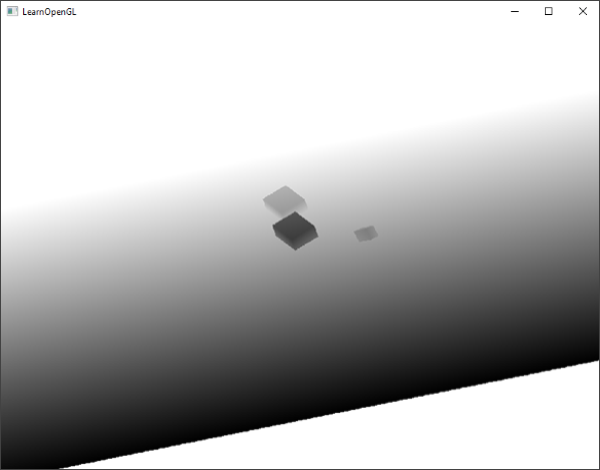
\includegraphics[width=0.7\textwidth]{img/shadow_mapping_depth_map.png}
    \caption{Visualizzazione della depth/shadow map memorizzata nel buffer}
\end{figure}

\section{Renderizzare la scena con le ombre}
Ottenuta la depth map possiamo passare a renderizzare la scena con le nostre ombre, apportando dei cambiamenti agli shader utilizzati finora per renderizzare la scena. Nel vertex shader aggiungiamo il calcolo del vettore FragPosLightSpace, ovvero il vettore della posizione dello spazio mondo trasformato nello spazio luce, il quale viene mandato in input al fragment shader.

\begin{minted}[bgcolor=black]{glsl}
vs_out.FragPosLightSpace = lightSpaceMatrix * vec4(vs_out.FragPos, 
                                                   1.0);
\end{minted}

Nel fragment shader, dove utilizziamo il modello di lighting di Blinn-Phong, aggiungiamo il calcolo delle ombre e modifichiamo il calcolo del vettore \textit{lightning}.

\begin{minted}[bgcolor=black]{glsl}
float shadow = ShadowCalculation(fs_in.FragPosLightSpace);
\end{minted}

Il valore restituito dalla funzione \textit{ShadowCalculation} (ne parleremo dopo) è un float compreso tra 0.0 (ovvero il frammento non è in ombra) e 1.0 (il frammento è totalmente in ombra). Questo valore viene utilizzato nel calcolo del lighting dove viene moltiplicato con i componenti della luce diffuse e specular; l'ambient viene escluso in quanto le ombre non sono mai completamente nere a causa dello scattering della luce.

\begin{minted}[bgcolor=black]{glsl}
vec3 lighting = (ambient + (1.0 - shadow) * (diffuse + specular)) 
                 * color;
\end{minted}	

La funzione ShadowCalculation prende la profondità del frammento corrente nello spazio luce e la confronta con closestDepth, ovvero la profondità del frammento più vicino sulla retta tra la fonte di luce e il frammento corrente campionata dalla shadow map; se la profondità del frammento corrente è maggiore di currentDepth, restituisce 1, altrimenti 0.\\
La funzione è così definita:

\begin{minted}[bgcolor=black]{glsl}
float ShadowCalculation(vec4 fragPosLightSpace)
{
    vec3 projCoords = fragPosLightSpace.xyz / fragPosLightSpace.w;
    projCoords = projCoords * 0.5 + 0.5;
    float closestDepth = texture(shadowMap, projCoords.xy).r; 
    float currentDepth = projCoords.z;
    float shadow = currentDepth > closestDepth  ? 1.0 : 0.0;

    return shadow;
}
\end{minted}

Il risultato del secondo rendering (ovvero della scena) è il seguente:

\begin{figure}[H]
    \centering
    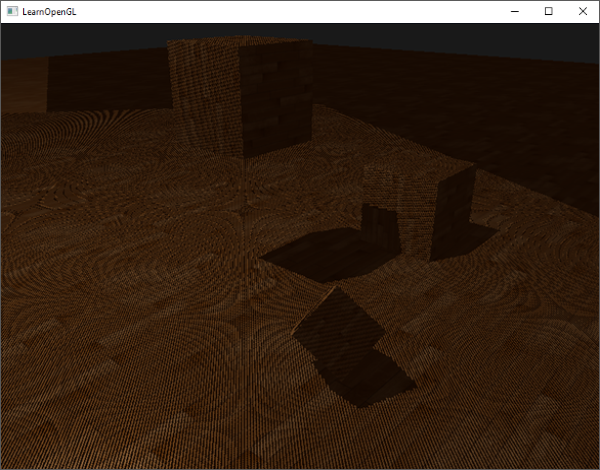
\includegraphics[width=0.8\linewidth]{img/shadow_mapping_shadows.png}
    \caption{Risultato del secondo rendering}
\end{figure}

\chapter{Problemi}
Nel risultato finale possiamo notare che le ombre sono state generate, ma sono presenti diversi problemi.

\section{Shadow acne}
Il primo problema (e quello più evidente) è un pattern di linee nere sul pavimento. 

\begin{figure}[H]
    \centering
    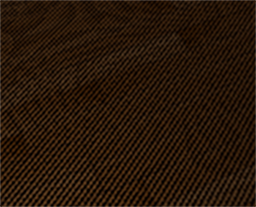
\includegraphics[scale=0.5]{img/shadow_mapping_acne.png}
\end{figure}

Questo artefatto è chiamato shadow acne e può essere spiegato con la seguente immagine:

\begin{figure}[H]
    \centering
    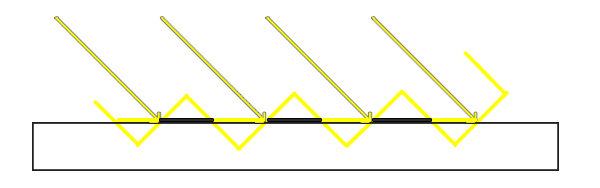
\includegraphics[width=0.5\linewidth]{img/shadow_mapping_acne_diagram.png}
\end{figure}

Quando i raggi di una fonte di luce colpiscono una superficie con un'angolazione non perpendicolare, molti frammenti (quando sono relativamente distanti dalla fonte di luce) accedono allo stesso texel di profondità che potrebbe risultare sopra per alcuni o sotto alla superficie per altri; questo porta ad una discrepanza nell'ombra.

\begin{figure}[H]
        \centering
        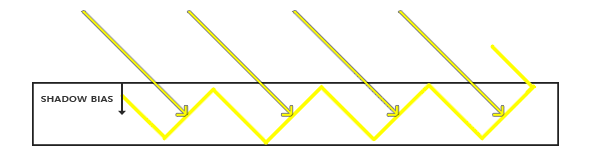
\includegraphics[width=0.5\textwidth]{img/shadow_mapping_acne_bias.png}
        \caption{applicando il bias}
\end{figure}
La soluzione consiste nell'aggiungere un bias alla profondità corrente (o alla shadow map) affinchè i frammenti non siano considerati sopra la superficie. Questo metodo è chiamato \textbf{shadow bias}



\begin{figure}[H]
        \centering
        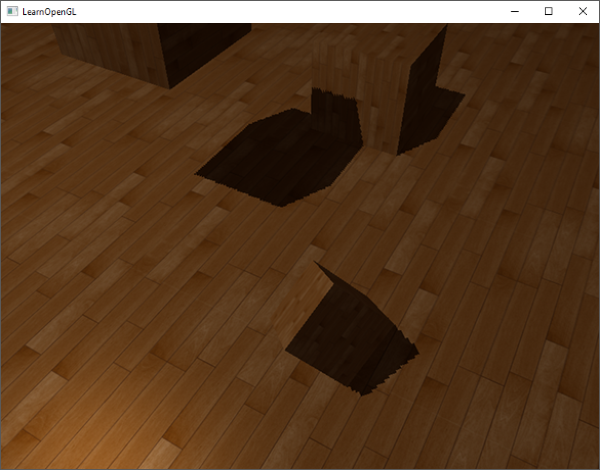
\includegraphics[width=0.5\textwidth]{img/shadow_mapping_with_bias.png}
        \caption{Applicando il bias al nostro esempio}
\end{figure}

\section{Peter panning}
Uno svantaggio dell'applicare lo shadow bias è l'applicazione di un offset alla profondità effettiva delle ombre, facendole apparire distaccate dagli oggetti (da qui il nome \textbf{peter panning})

\begin{figure}[H]
    \centering
    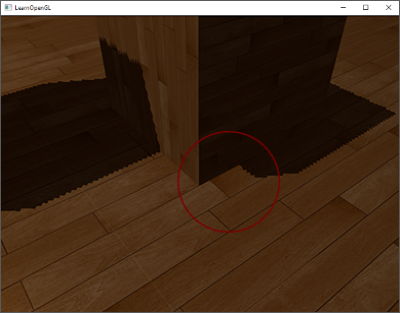
\includegraphics[width=0.5\linewidth]{img/shadow_mapping_peter_panning.png}
    \caption{Esempio di peter panning applicando un bias esagerato}
\end{figure}

Per risolvere questo problema si genera la shadow map utilizzando il retro delle facce degli oggetti.

\begin{figure}[H]
    \centering
    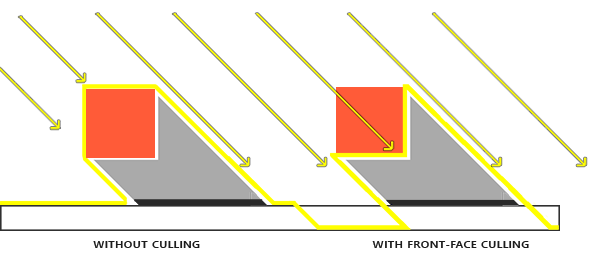
\includegraphics[width=1.0\linewidth]{img/shadow_mapping_culling.png}
\end{figure}

In OpenGL chiamiamo la funzione GL\_CULL\_FACE() con argomento GL\_FRONT per abbattere le facce frontali per il calcolo della depth map, ripristinandole successivamente per il rendering della scena normale.

Questo metodo può essere applicato solo per oggetti solidi che non hanno aperture verso l'interno. Inoltre non funziona sui single plane (il nostro pavimento per esempio), poiché sarebbero abbattuti. 

Oggetti troppo vicini alla fonte di luce potrebbero dare ancora risultati non corretti.

Tuttavia il fenomeno del peter panning è evitabile utilizzando bias piccoli.

\section{Aliasing}
Se zoomiamo sull'ombra possiamo vedere come questa è affetta da aliasing, ovvero sul bordo dell'ombra c'è una transizione netta tra ombra e luce, risultando sgradevole alla vista.

\begin{figure}[h]
    \centering
    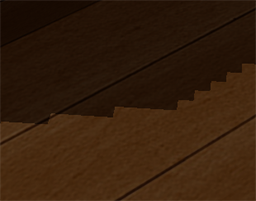
\includegraphics{img/shadow_mapping_zoom.png}
\end{figure}

Ci sono varie soluzioni parziali all'aliasing, tra queste aumentare la risoluzione della texture dell'ombra e/o avvicinare il più possibile il tronco di luce alla scena.

Un'altra soluzione parziale al problema dell'aliasing si chiama \textbf{PCF}, ovvero percentage-closer filtering, un set di funzioni di filtraggio che producono ombre più morbide. L'idea è quella di campionare più volte la depth map ogni volta con piccole variazioni nelle coordinate della texture. Per ogni campione controlliamo se questo è in ombra o meno. Una volta terminato facciamo la media di tutti i campioni e otteniamo l'ombra.

\begin{figure}[H]
     \centering
     \begin{subfigure}[b]{0.7\linewidth}
         \centering
         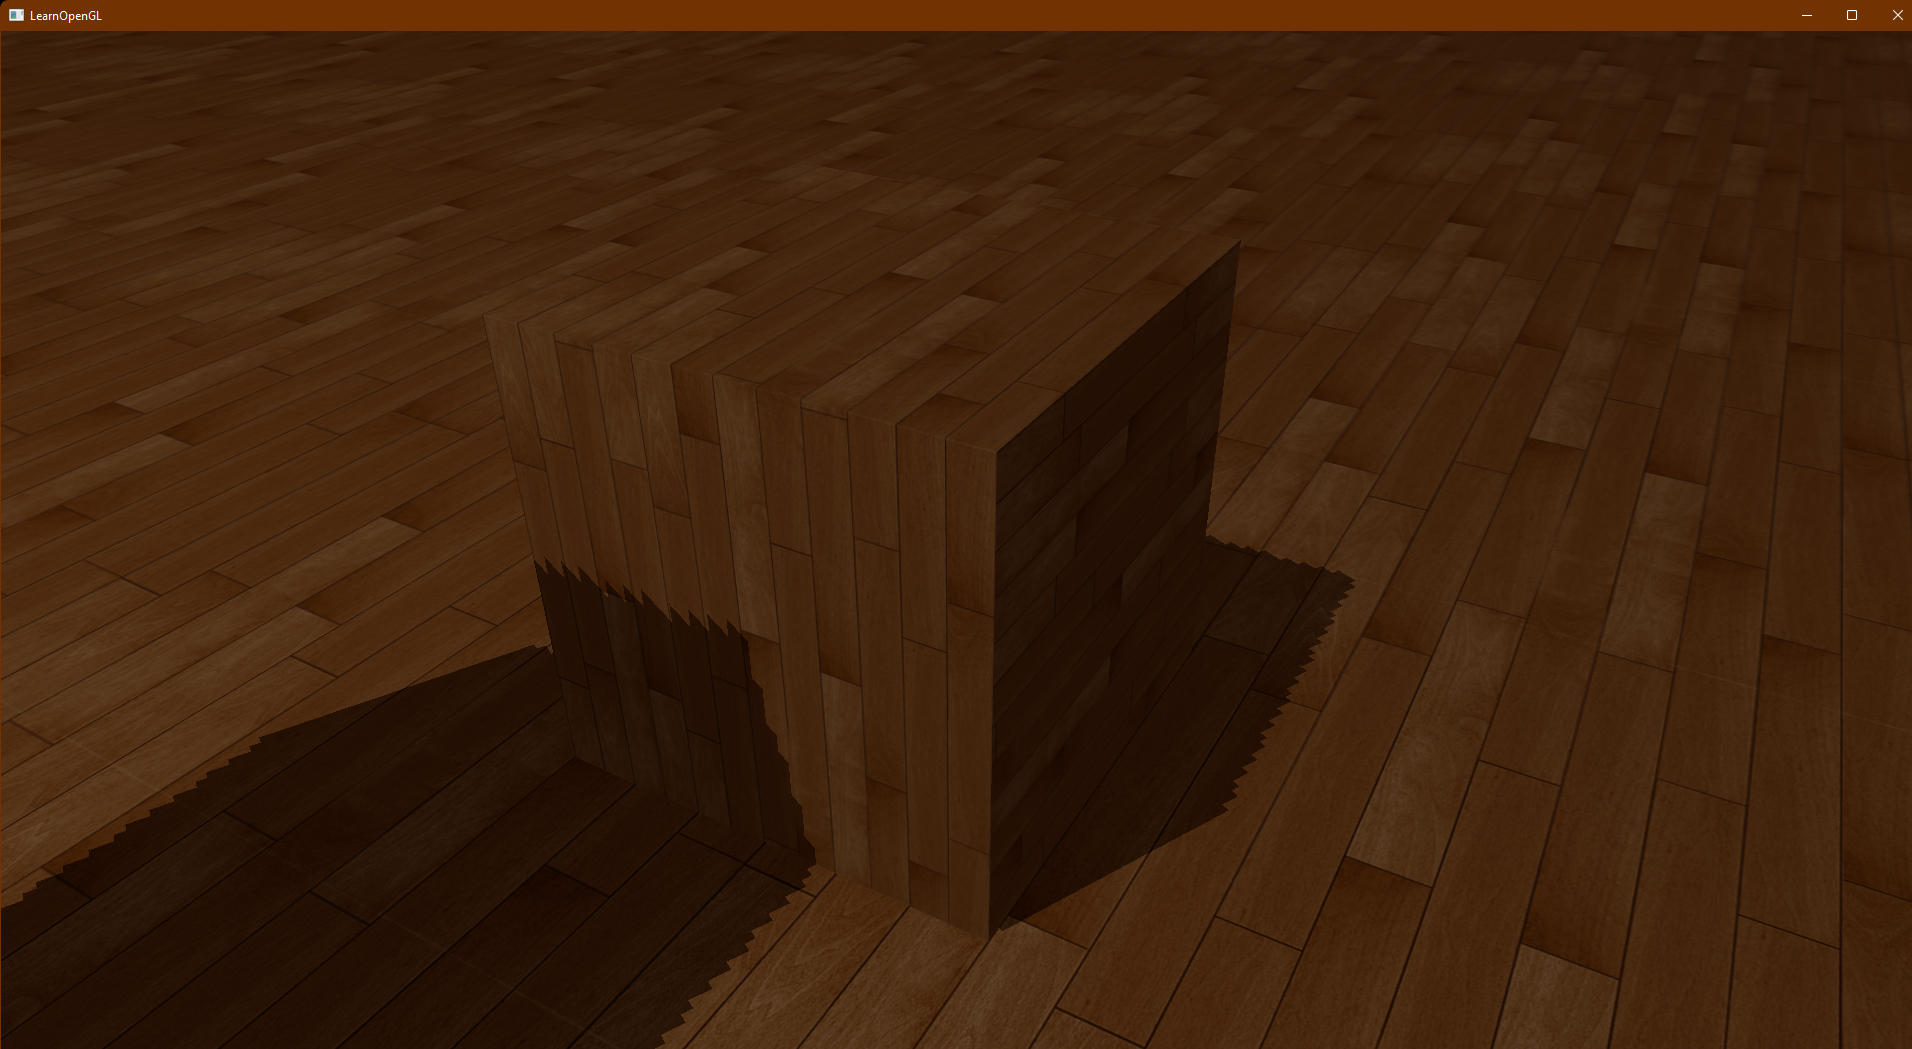
\includegraphics[width=\linewidth]{img/LearnOpenGL 23_09_2021 17_16_24.png}
         \caption{Prima}
     \end{subfigure}
     \begin{subfigure}[b]{0.7\linewidth}
         \centering
         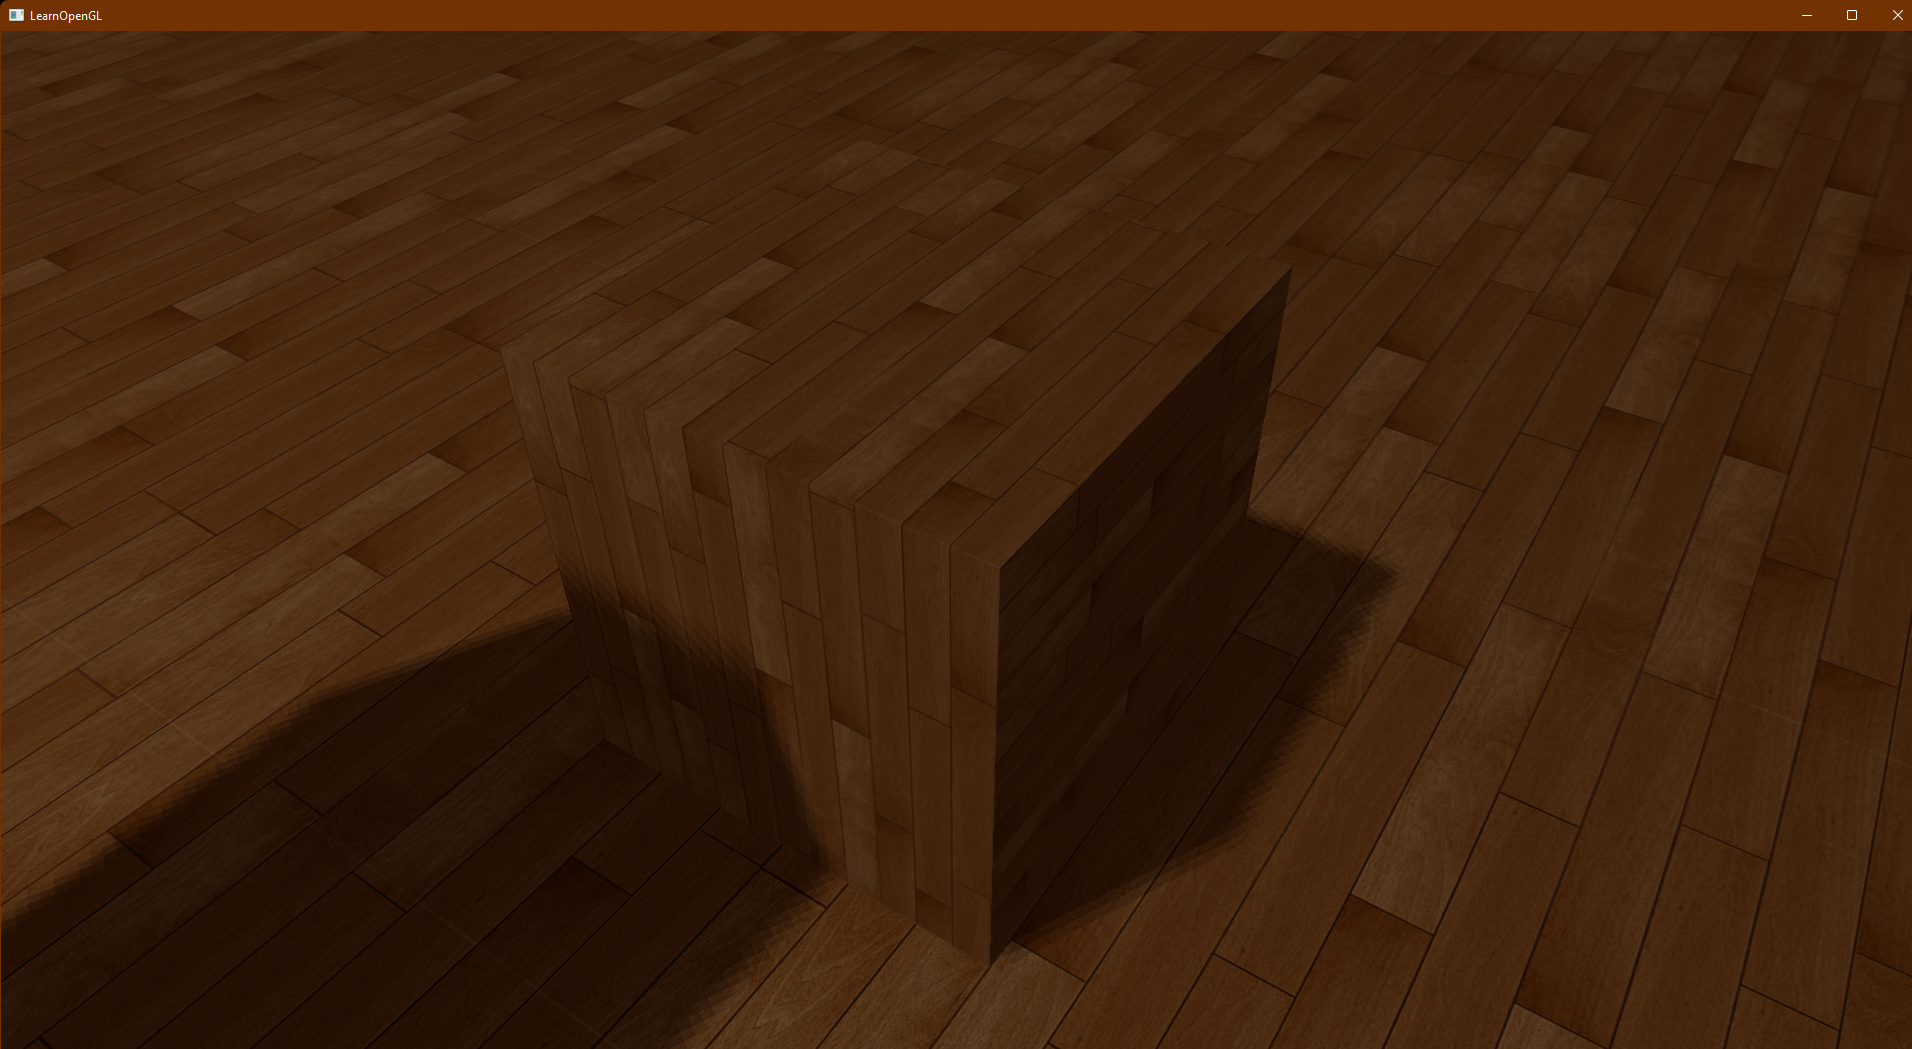
\includegraphics[width=\linewidth]{img/LearnOpenGL 23_09_2021 17_16_58.png}
         \caption{Dopo}
     \end{subfigure}
\end{figure}

Una semplice implementazione in OpenGL è la seguente:

\begin{minted}[bgcolor=black]{glsl}
float shadow = 0.0;
vec2 texelSize = 1.0 / textureSize(shadowMap, 0);
for(int x = -1; x <= 1; ++x)
{
    for(int y = -1; y <= 1; ++y)
    {
        float pcfDepth = texture(shadowMap, projCoords.xy 
                                 + vec2(x, y) * texelSize).r; 
        shadow += currentDepth - bias > pcfDepth ? 1.0 : 0.0;        
    }    
}
shadow /= 9.0;
\end{minted}

\end{document}